\documentclass{training}

\title{3D Printing}
\date{\today}
\author{Blaise Thompson}

\begin{document}

\maketitle
\renewcommand{\baselinestretch}{0.5}\normalsize
\tableofcontents
\renewcommand{\baselinestretch}{1.0}\normalsize
\vfill

Part of the training materials prepared by the \href{https://shops.chem.wisc.edu/}{Chemistry Shops} at UW--Madison. \\
Source code and all associated files can be found at \href{https://github.com/uw-madison-chem-shops/training}{GitHub}. \\
If you find any mistakes or feel that any information is missing, please \href{https://github.com/uw-madison-chem-shops/training/issues}{open an issue}. \\

\clearpage
\section{Options}

\begin{center}
\begin{tabular}{ l | l | l | l }
 material & cost & melting point & comment \\ \hline
 ABS & $\$5.00 / \mathrm{in}^3$ & 220\textcelsius & self-service \\
 ASA & $\$3.50 / \mathrm{in}^3$ & 240\textcelsius & via UW Makerspace \\
 PLA & $\$2.00 / \mathrm{in}^3$  & 160\textcelsius & via UW Makerspace \\
 Nylon & ??? & 220\textcelsius & UW Makerspace. Scintillated.
\end{tabular}
\end{center}

To print via the UW Makerspace, contact Blaise Thompson.
A flat fee of $\$7$ will be added to the cost of material for any non self-service print.

\section{Self-Service Printing}

\begin{enumerate}
    \item Generate STL file, units mm. Bring to control computer.
    \item Turn on 3D printer.
    \item Ensure build plate is clean and correctly installed.
    \item Open Catalyst EX.
    \item File, Open STL.
    \item Choose layer resolution, interior fill.
    \item Pack. Note sum of model + support material volume. Bill yourself out.
    \item Print.
    \item On printer, press ``start model''.
    \item Wait until printer actually begins printing (30 minutes).
    \item If long print, leave ``This eqipment being used'' card.
    \item You are responsible for picking up your print.
\end{enumerate}

\section{3D Printing Design Tips}

Press-fit 4-40 tapped holes.

Use hexagonal or tear-dropping holes.

\clearpage

Restocking parts.

We buy parts from \href{https://www.shop.h2igroup.com/}{H2I Group}.
Relevant part numbers follow.

\begin{center}
\begin{tabular}{ l | l | r }
 description & part number & cost (\$) \\ \hline
 WaterWorks Soluble Concentrate P400-SC (case of 12) & 300-00600 & 165.00  \\
 Ecoworks Cleaning Agent (case of 24) & 300-00103 & 165.00 \\ \hline
 Ivory Filament (42 cubic inches) & 345-42005 & 125.00 \\
 Black Filament (42 cubic inches) & 345-42006 & 125.00 \\
 Dark Grey Filament (42 cubic inches) & 345-42007 & 125.00 \\
 Red Filament (42 cubic inches) & 345-42008 & 125.00 \\
 Blue Filament (42 cubic inches) & 345-42009 & 125.00 \\
 Nectarine Filament (42 cubic inches) & 345-42010 & 125.00 \\
 Fluorescent Yellow Filament (42 cubic inches) & 345-42011 & 125.00 \\
 Olive Green Filament (42 cubic inches) & 345-42012 & 125.00 \\
 White Filament (42 cubic inches) & 345-42100 & 125.00 \\
 Soluble Support (42 cubic inches) & 345-42207 & 225.00 \\ \hline
 Modeling Bases (pack of 24) & 340-00200 & 140.00 \\
 Tip Replacement Kit & 540-00900 & 150.00
\end{tabular}
\end{center}

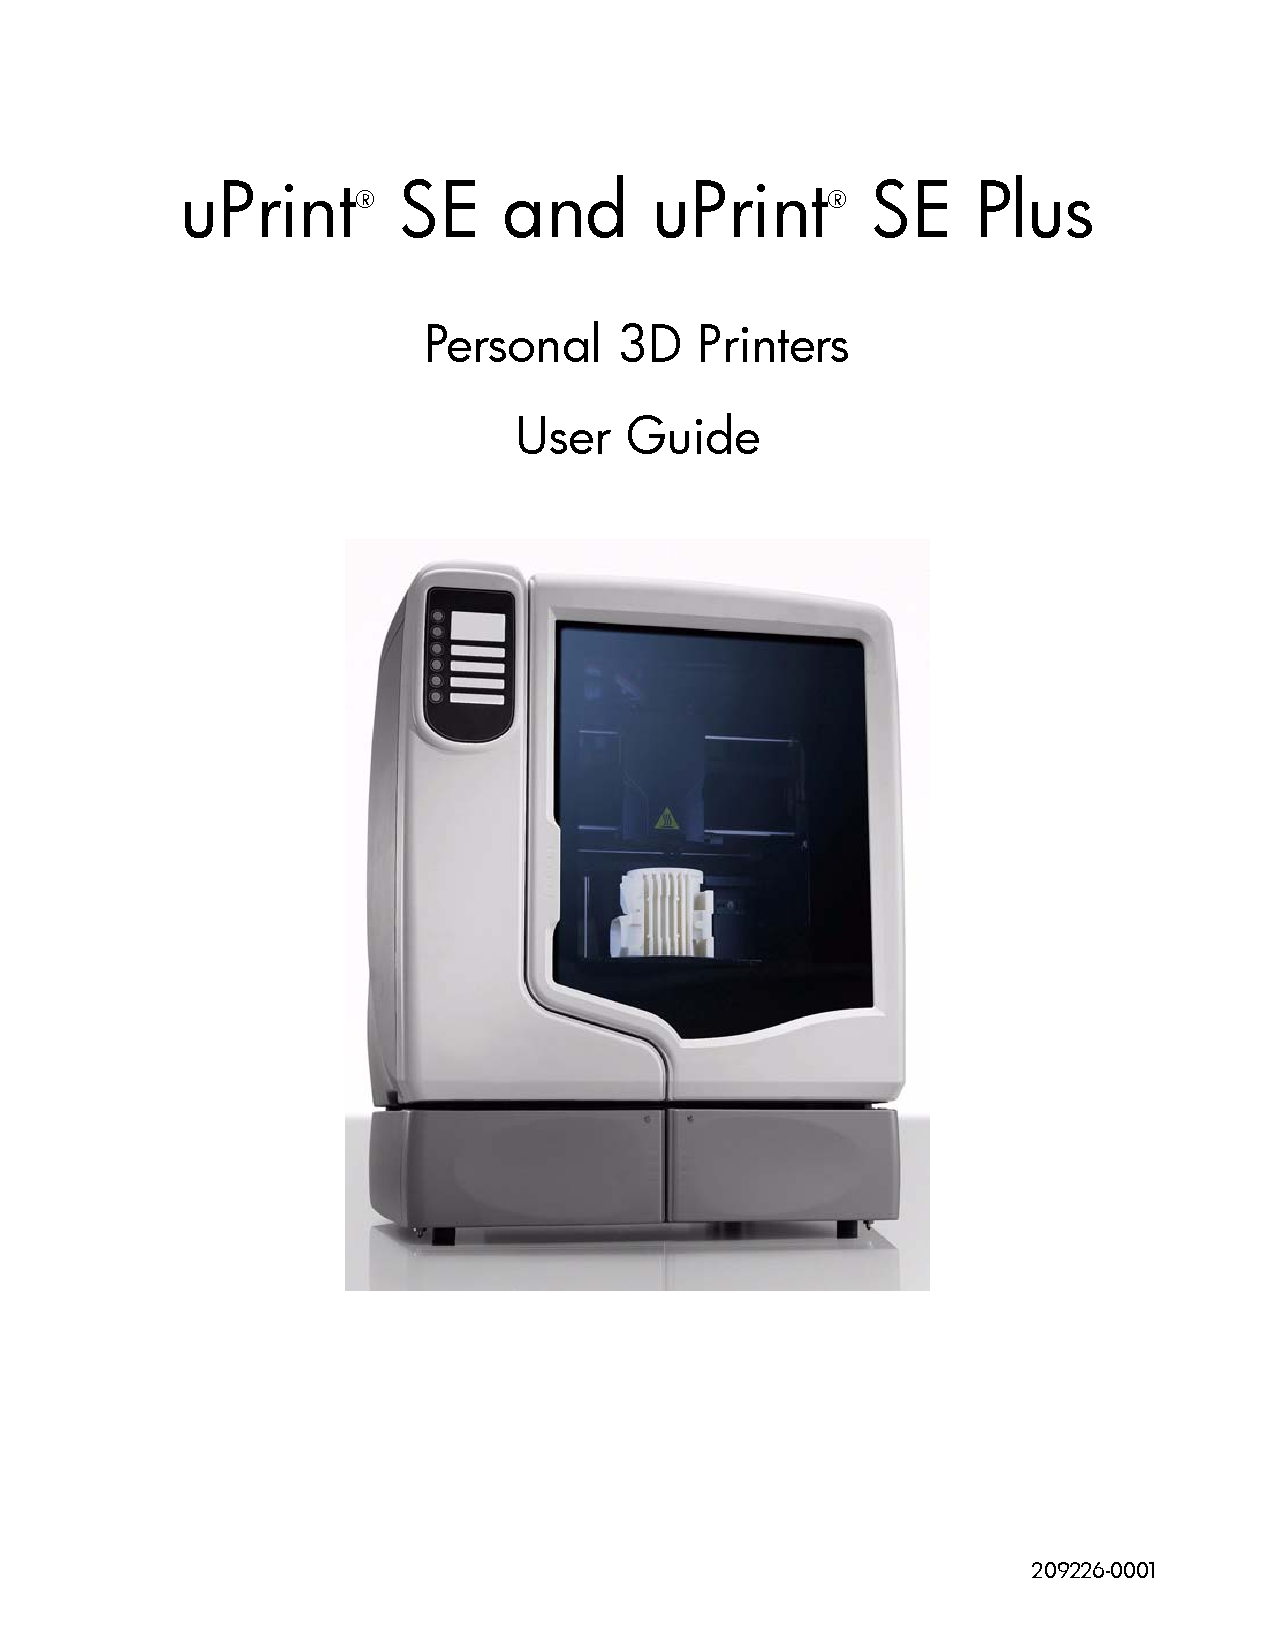
\includepdf[pages=-]{UprintSE_3Dprinter_Manual.pdf}

\end{document}
